\documentclass[review]{elsarticle}

\usepackage[]{geometry}
\usepackage{amsmath}
\usepackage{tikz}
\usepackage[nomessages]{fp}
\usepackage{graphicx}
\usepackage{hyperref}
\usepackage{natbib}
\bibliographystyle{elsarticle-harv}
\biboptions{authoryear}

\newcommand{\drawcirclerow}[5][0] { % args: [start], count, color, height, radius
  \FPadd\stop#2#1
  \foreach \i in {#1,...,\stop} {
    \ifnum \i < \stop
    \fill[#3] (\i, #4) circle (#5);
    \draw (\i, #4) circle (#5); 
    \fi
  }
}

\newcommand{\ra}{\rightarrow}
\newcommand{\sgcomment}[1]{\textcolor{red}{SG: #1}}
\newcommand{\ikcomment}[1]{\textcolor{blue}{IK: #1}}


\journal{Theoretical Population Biology}

\begin{document}
\begin{frontmatter}
  \title{Counting parental contribution - how large sample size makes strong selection weak}

  \author{Ivan Krukov}
  \author{Simon Gravel}

  \begin{abstract}
    Neutral models of genetic diversity tend to be easier to analyze compared to models including
    selection. Because lineages are exchangeable in the neutral Wright-Fisher model, for example,
    the number of lineages that are relevant to the ancestry of a sample at a single locus can only
    decrease as we go back in time. As a consequence, useful recursion equations can be derived for
    patterns of polymorphism. By contrast, under negative selection, the number of relevant lineages
    can increase as we go back in time, and the equivalent recursion equations do not close. Given a
    large enough sample size, however, the reduction in the number of lineages due to genetic drift
    is larger than the increase in the number of lineages due to natural selection, and the number
    of relevant lineages is unlikely to increase. We use this observation to derive asymptotically
    closed recursion equations for the distribution of allele frequencies. We show that this
    approach is accurate under strong drift and strong natural selection. We derive several
    asymptotic results to understand when the sample size is sufficiently large to overcome the
    influence of selection.
    
  \end{abstract}
\end{frontmatter}

\section{Introduction}
\label{sec:introduciton}

The calculation of the allele frequency spectrum (\textit{AFS}) is an important tool for the inference
of demographic histories and other population genetic parameters. In the absence of selection, the
number of parental lineages that contribute to the sample decreases back in time due to coalescent
events. This means that the equations are closed with respect to the sample size under neutrality.
This has paved the way for moment-based recursions of the allele frequencies
\citep{KimuraCrow1964,Ewens1972,DonnellyKurtz1999}. Recently, a number of successful methods,
including \citep{GutenkunstEtAl2009,JouganousEtAl2017,KammEtAl2017}, have become popular for this
purpose. At their core, these methods describe the time-evolution of the \textit{AFS}. The goal of
these approaches is to obtain the probability of observing a given number of derived alleles in a
finite sample conditional on the state of the parental lineages.

Despite many successes, considering selection has been problematic within this framework. Under
negative selection, the number of parental lineages that contribute to a sample can be larger that
the sample size itself, due to selective death events. As a consequence, the equation lose the
closure property \citep{JouganousEtAl2017}.

An extension to the Kingman's coalescent \citep{Kingman1982a}, the ancestral selection graph
(\textit{ASG}), \citep{KroneNeuhauser1997} considers the ancestry of a sample in the presence of
selection. The \textit{ASG} framework can be used to study the ancestry of highly deleterious
alleles \citep{Wakeley2009} under certain assumptions. Another possible resolution is to use an
uncontrolled jackknife approximation to add extra lineages - the method proposed in
\citep{JouganousEtAl2017}.

Unlike the \textit{ASG}, the present method does not need to assume an infinitely large population
size, and also explicitly tracks multiple coalescent events, which is important with large sample
sizes \citep{BhaskarEtAl2014}. Our approach can also be combined with the jackknife. Unlike the
jackknife, our method allows derivation of bounds on the performance of the approximation.

\section{Background}
\label{sec:background}

Consider the behavior of a single biallelic locus in a haploid Wright-Fisher model with a population
of size $N$. We consider a sample of size $n$ lineages from within the population. We want to know
how many parental lineages $r$ have contributed to the present sample from one generation in the
past. Going back in time, the random variable $\mathcal{R}$ is the number of lineages that
contribute to the present day sample. Figure \ref{fig:schematic} shows examples the different models
that we consider below -- standard coalescent (\ref{fig:schematic}A), coalescent with multiple
merges (\ref{fig:schematic}B), and coalescent with multiple merges and selection
(\ref{fig:schematic}C).

\begin{figure}[ht]
  \centering
  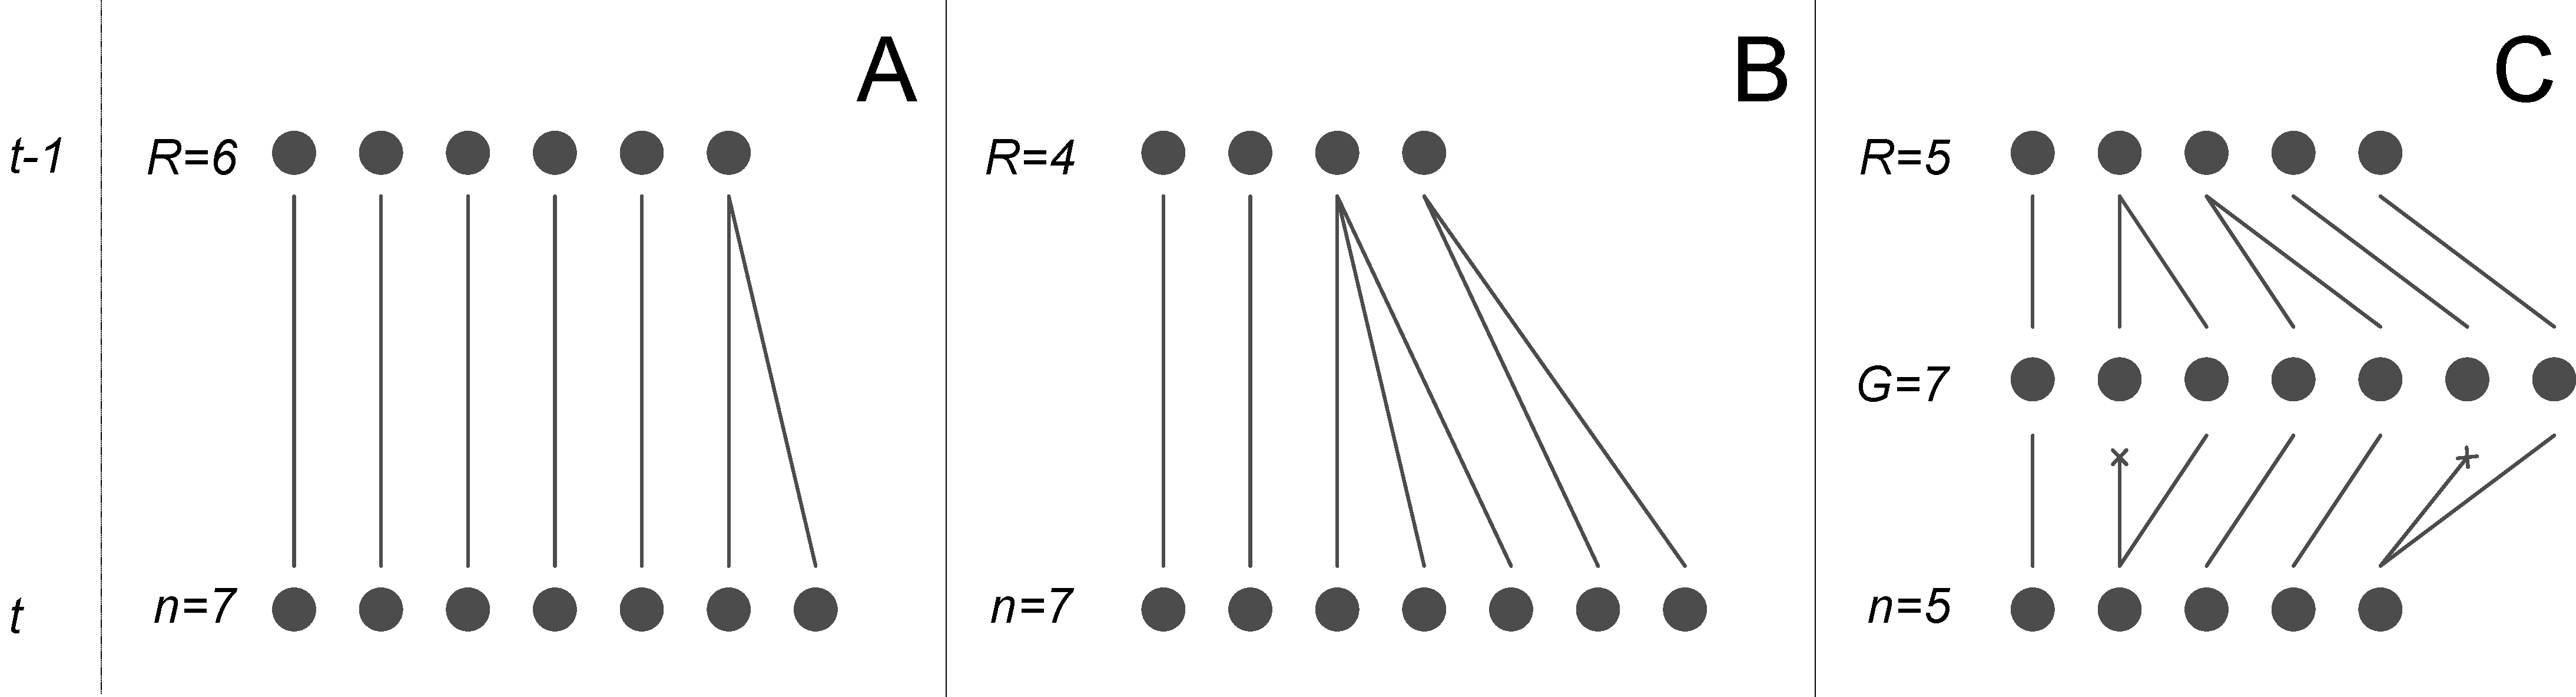
\includegraphics[width=0.8\textwidth]{fig/schematic.pdf}
  \caption{\label{fig:schematic} Realizations of sampling models, showing $\mathcal{R}=r$ parental
    lineages at $t-1$ contributing to $n$ lineages in present generation $t$. \textbf{A} Standard
    coalescent - at most 1 coalescent event per generation; $r\in[n-1, n]$. \textbf{B} Coalescent
    with multiple merges - parents \textit{3} and \textit{4} have 3 and 2 offspring, respectively;
    $r \in [1, n]$ \textbf{C} Including selection - each parent produces a random number of gametes
    ($\mathcal{G}$), which then may survive to produce offspring; $r \in [1, n]$, $g \in [n, 2n]$ }
\end{figure}

First, consider a recursion describing the evolution of the expected allele frequency spectrum
(\textit{AFS}) $\Phi_{n}^{(t)}$, in the standard coalescent without selection (Figure
\ref{fig:schematic}A). At generation $t$, the sample consists of $n$ lineages, and at $t-1$ there
are $r$ parental lineages. In what follows, we closely follow the exposition of
\cite{JouganousEtAl2017}. The standard coalescent model allows at most one event per generation, so
we need to consider only two cases: namely $r=n$ if no coalescent occurs, and $r=n-1$ if a single
event took place.

Without a coalescent event, $r$ parental lineages are sampled randomly into the present generation,
so the allele frequencies remain the same: $\Phi_{n}^{(t)}=\Phi_{n}^{(t-1)}$. With a single
coalescent event, the contribution comes from $r=(n-1)$ parental lineages:
$\Phi_{n}^{(t)}=\mathcal{D}\Phi_{n-1}^{(t-1)}$, where $\mathcal{D}$ is a sparse $n \times (n-1)$
matrix describing the effect of drift. We do not use $\mathcal{D}$ in this work (but see
\citep{JouganousEtAl2017}), and instead construct a related matrix in section \ref{subsec:markov}.
Combining the terms without and with the coalescent event, we have:

\begin{align}
  \label{eq:op-neutral}
  \Phi_{n}^{(t)}=\Phi_{n}^{(t-1)}+\mathcal{D} \Phi_{n-1}^{(t-1)}
\end{align}

In other words, the \textit{AFS} of size $n$ at time $t$ can be obtained if we know the \textit{AFS}
of sample sizes $n$ and $n-1$ in the previous generation. This gives rise to a recursion formula for
the frequency spectrum that can be solved efficiently \citep{JouganousEtAl2017}. Here we would like
to generalize such an approach to cases including natural selection and large sample sizes.

We first incorporate the effects of large sample size. As previously shown in
(\cite{BhaskarEtAl2014} and \cite{NelsonEtAl2019}), the coalescent approximation may not be adequate in this
setting, since multiple coalescent events can take place within a single generation
(Figure \ref{fig:schematic}B). With a slight abuse of notation we denote $\mathcal{D}_i$ as the
$i^{\text{th}}$-order drift matrix in which $i$ lineages are lost due to genetic drift. The
dimensionality of $\mathcal{D}_i$ is $n \times (n-i)$. For example, $\mathcal{D}_2$ includes both
three-way coalescent and double two-way coalescent. In section \ref{subsec:markov}, we demonstrate an
efficient dynamic programming algorithm to exhaustively enumerate all the events for a drift-only
model.

With multiple coalescent events per generation, \eqref{eq:op-neutral} becomes:

\begin{align}
  \label{eq:op-neutral-mult}
  \Phi_{n}^{(t)}=\Phi_{n}^{(t-1)}+\sum_{i=1}^{n}\mathcal{D}_i \Phi_{n-i}^{(t-1)}
\end{align}

The equation \eqref{eq:op-neutral-mult} is still closed in terms of the sample size, since
$\Phi_{n}^{t}$ only depends on $r=(n-i)<n$ parental lineages. 


If we now consider selective death events, we must also account for lineages that were not
transmitted due to selection. We use the model shown in figure \ref{fig:schematic}C to describe
this. Each generation, a random number of $\mathcal{R}=r$ parental lineages produce a large number
of gametes, $\mathcal{G}=g$. Then $n$ individuals are formed by randomly sampling gametes, without
replacement. The probability of successfully sampling a particular gamete is $1-xs$, where $x$ is
the frequency of the derived allele in the parental generation. In the case of a selective death a
new lineage is re-drawn with probability $xs$. This sampling scheme allow us to consider drift ($r
\ra g$) and selection ($g \ra n$) within the same generation as distinct processes.
\ikcomment{Should we use $s$ or $s/1+s$?}
 
For example, in case of a single selective death event, we have
$\Phi_{n}^{(t)}=\mathcal{S}\Phi_{n+1}^{(t-1)}$, with selection matrix $\mathcal{S}$. Multiple
selection events are possible per generation, but we restrict our attention to the case where each
lineage experiences at most one selective death event. This still allows us to consider strong
selection, with at most $r\le 2n$ parental lineages contributing:

\begin{align}
  \label{eq:op-selection}
  \Phi_{n}^{(t)}=\Phi_{n}^{(t-1)}+ \sum_{j=n}^{2n} \sum_{i=1}^{n} \mathcal{S}_j \mathcal{D}_i \Phi_{n-i+j}^{(t-1)}
\end{align}

The closure no longer holds for \eqref{eq:op-selection}, as up to $2n$ gametes can contribute to the
sample. However, the effect of a large sample size counteracts the additional lineages needed due to
selection. The opposite effects of drift and selection on the number of lineages relevant to a
sample are particularly clear in the context of the size of the ancestral selection graph
(\textit{ASG}): in which the number of lineages relevant to a sample can be described as a
birth-death process \citep{KroneNeuhauser1997, Wakeley2009}:

\begin{align}
  \label{eq:asg-size}
  n \ra \begin{cases}
    n+1 & \text{at rate } Ns \frac{n}{2} \hspace{20pt} \text{ (selection) }\\
    n-1 & \text{at rate } \frac{n(n-1)}{2}   \hspace{28pt} \text{ (coalescence) }
  \end{cases}
\end{align}

The coalescence (drift) term is quadratic with respect to the sample size, while the selection term
is linear. The rate of coalescence is higher than the rate of selective deaths if the number of
lineages $n>Ns+1$.

Our goal here is to define recursions generalizing equation \eqref{eq:op-neutral}. For the equations
to be closed, we need to ensure that the rate of coalescence is large enough that it overcomes the
rate of selection not only on average, but \emph{almost always}.

The rest of the paper is organized into two sections. In the first section, we construct a Markovian
recursion to track the number of derived lineages in a large sample from a Wright-Fisher model,
similar to \citep{JouganousEtAl2017,KammEtAl2017}. In this, we fully account for multiple coalescent
events per generation, and show that we restore closure with increasing sample size. In the second
part, we derive a number of asymptotic results to get a better understanding of the process. We
construct an exact probability distribution for the number of contributing parental lineages,
together with several approximations. Importantly, we derive a normal approximation that allows us
to calculate a quantile of the sample size where the system is approximately closed.

\section{Results}
\label{sec:results}

\subsection{Markov process construction}
\label{subsec:markov}

We first define a recursion equation for the distribution of allele frequency in a sample of size
$n$ from a haploid Wright-Fisher population of size $N$. Given that the sample in parental generation
has $j$ copies of the derived allele, we seek to calculate the probability that the sample
will contain $i$ derived copies in the following generation.

In the neutral case, this transition probability can be calculated if we know the transition
probabilities in the smaller samples of size $n' \in [1, n-1]$ (similar to
\eqref{eq:op-neutral-mult}) \citep{BhaskarEtAl2014}. We do not construct the intermediate matrices
$\mathcal{D_i}$ of \eqref{eq:op-neutral-mult} explicitly, but instead calculate a matrix
$P((j,n)\ra(i,n))$, giving the probabilities of transitioning from $j$ to $i$ derived alleles in
sample of size $n$ within one generation. In brief, we can construct the transition probability
matrix $P((j,n)\ra(i,n))$ if we know the matrix for $n-1$, $P((\cdot,n-1)\ra(\cdot,n-1))$, and then
use the conditional probabilities for each type of an event. Starting from the base cases for a
sample size of $1$, we build up a set of square transition probability matrices. By using a dynamic
programming algorithm, we can achieve reasonable performance for realistic sample sizes. The full
derivation is shown in appendix A.

The case of selection is slightly more complicated, since now we need to consider a larger set of
states that can lead to transition from $j$ to $i$ copies in a sample size of $n$. In particular,
there can be a large number of gametes (fig. \ref{fig:schematic}C) that can contribute from $n$ when
there is no selection, to a potentially infinite number under strong negative selection. In our
calculation, we only consider up to one selective death event per lineage, so the number of
contributing gametes is between $n$ and $2n$.

Note that this is analogous to the outer summation boundaries in eq. \eqref{eq:op-selection}. Again,
we do not calculate the matrix $\mathcal{S}_i$ directly, but rather construct a transition
probability $Q((j,n)\ra(i,n))$. We can define these transitions recursively if we know the
transitions of $Q((\cdot,m)\ra(\cdot,n-1))$. Note that with selection we can have $m \in [1, 2n]$
lineages contribute, whereas we only needed $n' \in [1, n-1]$ in the neutral case.

To retain the closure property under selection, the Markov process needs to take $2n$ lineages in
the parental generation to $n$ lineages in the present. However, such rectangular transition
probability matrix is not suited for our purposes, since we want to describe the behavior of a
sample with constant size $n$. Instead, we only calculate the \textit{truncated} transition
probabilities for a $n \times n$ matrix $Q$. This means that under very strong selection, some
transitions will be unaccounted for. However, since the total sum of transition probabilities sums
to $1$, we can easily calculate the total missing probabilities. As we show in the rest of this
work, this missing probability tends to $0$ as sample size $n$ increases.

The construction of the full and truncated transition probability matrices is implemented via a
dynamic programming approach similar to the neutral case, and is described fully in
appendix B. Because we need to account for additional lineages in the selection case, the
calculation time is of the order of $O(n^4)$, while it is only $O(n^3)$ for the neutral case. The
increase in complexity makes this approach less suitable for large sample size, but we derive
several approximations in the following sections.

\subsection{Calculation of allele frequency spectra}
\label{subsec:afs}

Once the truncated matrix $Q$ is constructed, it can be used to calculate the allele frequency
spectrum. For the infinite sites model at equilibrium, we can calculate the \textit{AFS} $\Phi$ as a
solution to a linear system:

\begin{equation}
  \label{eq:sfs-calc}
  \Phi = \Phi Q + n \mu e_1
\end{equation}

where $\mu$ is the per-site mutation rate, and $e_1$ is the first column of the identity matrix of
size $n$. Figure \ref{fig:strong-selection} shows the comparison of the \textit{AFS} calculated from
Equation \eqref{eq:sfs-calc}, the diffusion approximation \cite[eq. 9.23]{Ewens2004}, and the
calculation performed in \texttt{Moments} \citep{JouganousEtAl2017}. Panel A shows a comparison at
$Ns=50$, with the population size ($N=2000$), which is substantially larger than the sample size
($n=200$). There is a small deviation between the approaches at large allele frequencies. At
stronger selection coefficients, \texttt{Moments} suffers from numerical instability, while the
diffusion approximation performs well (not shown).

If the sample size is the same as the population size ($n=N=200$) (Fig.
\ref{fig:strong-selection}B), the diffusion approximation and \texttt{Moments} perform poorly, while
our approach remains stable. This is expected, since the diffusion framework does not perform well
if multiple coalescent events contribute. Furthermore, if our sample size is the entire population,
we expect recursion equations to be closed. To confirm this, we compare our result to the
\textit{AFS} calculated from a whole-population haploid Wright-Fisher model, with $N=200$. (Fig.
\ref{fig:strong-selection}B) shows that our calculation is close to the full Wright-Fisher model.
The discrepancy between the curves is due to a difference in the way the selection coefficients are
calculated.

\begin{figure}
  \centering
  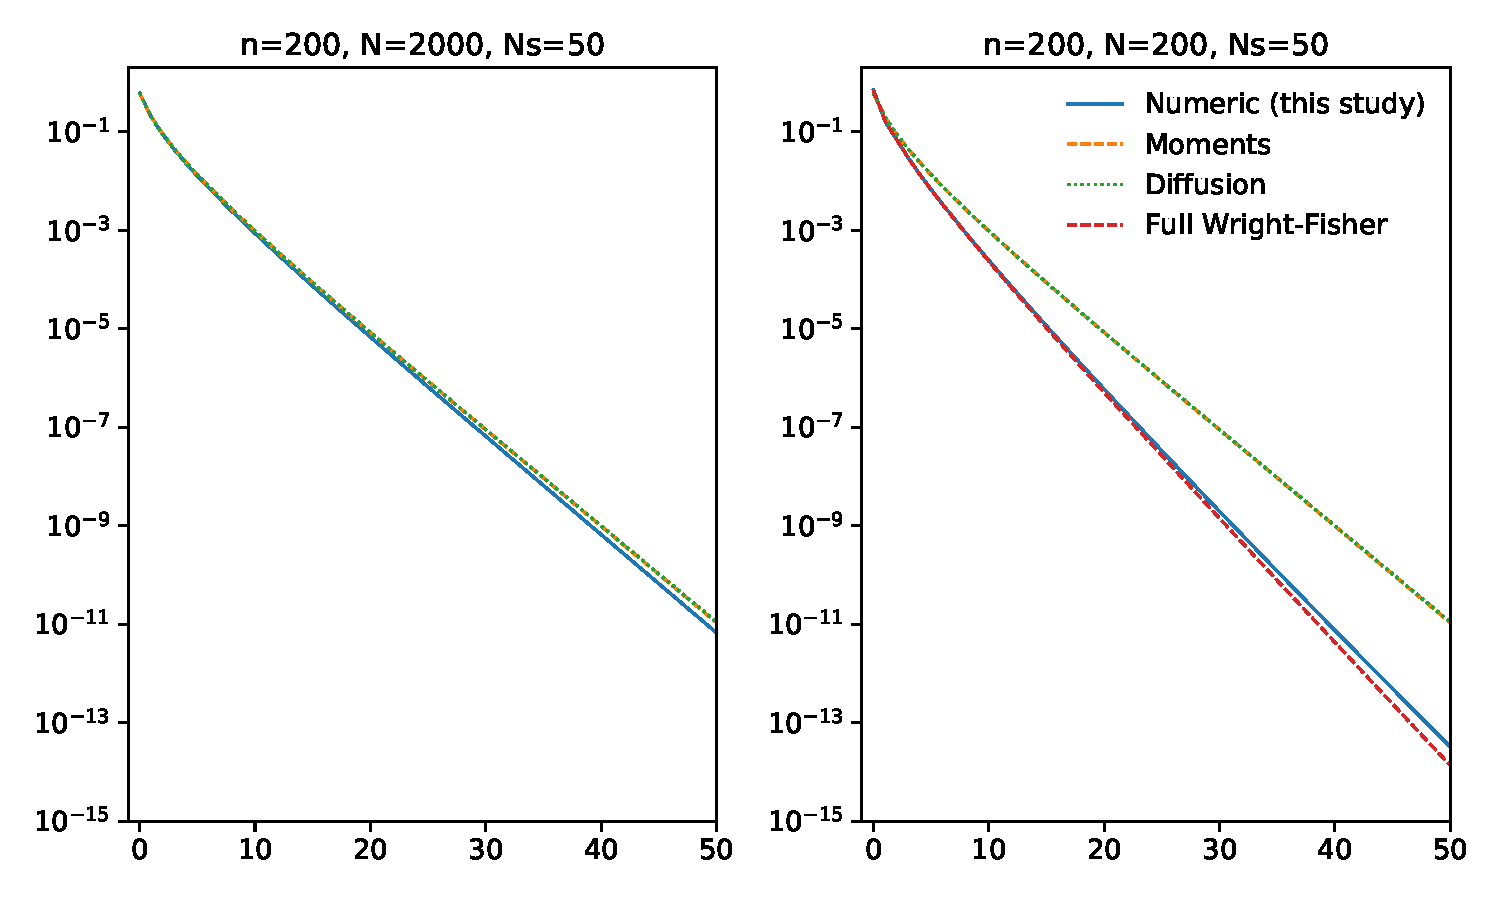
\includegraphics[width=0.7\textheight]{fig/strong_selection.pdf}
  \caption{Normalized allele frequency spectra in a sample of size $n=200$, for highly deleterious
    alleles ($Ns=-50$). (A) shows the frequency spectrum in a sample from a large population
    ($N=2000$), (B) in a small population ($N=200$). Both panels are truncated at $10^{-15}$, to
    show only moderately high allele frequencies.}
  \label{fig:strong-selection}
\end{figure}


\subsection{Closure properties}
\label{subsec:closure}

To show the closure properties of $Q$, we can calculate the total probability that more that $n$
parental lineages contribute to the sample of a given size. By construction, the sum of rows of $Q$
should correspond to the total probability mass that included configurations contribute (Fig.
\ref{fig:recurrence}). Thus, the probability that some number of configurations are unaccounted for,
with $j$ derived alleles in the parental sample, is given by $1-\sum_{i=0}^{n}Q_{i,j}$.
This probability depends on the number of derived alleles carried by the parental sample: the more
derived alleles, the higher the likelihood of a selective event. Figure \ref{fig:missing} shows the
probability of missing configurations in a sample size of $n=200$ in the worst-case scenario, with
$j=200$ derived lineages.

\begin{figure}
  \centering
  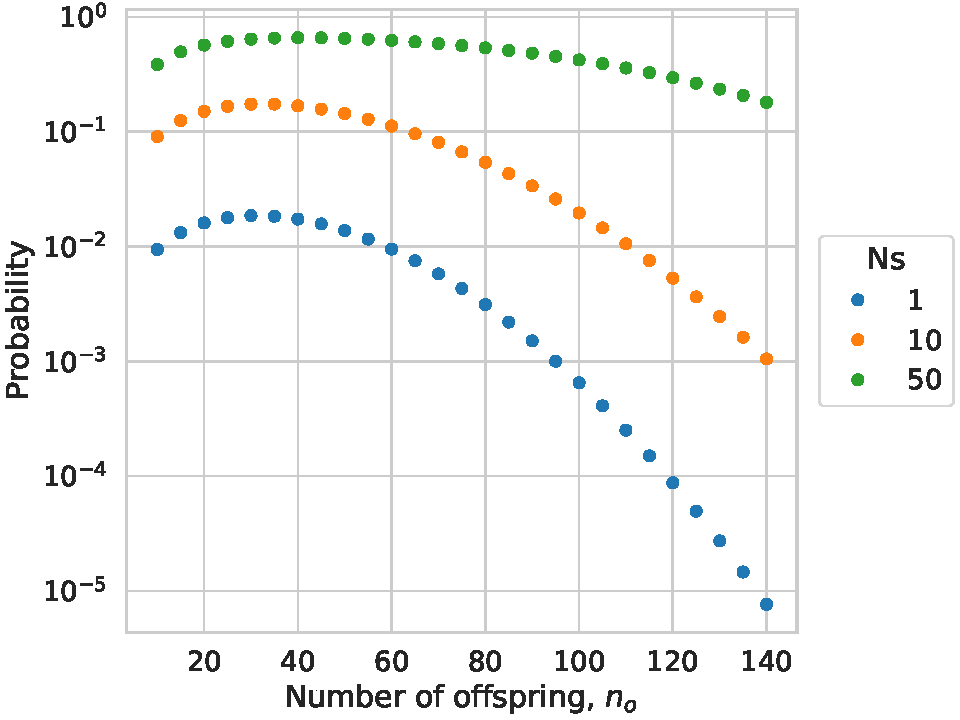
\includegraphics[]{fig/missing.pdf}
  \caption{Probability that unaccounted lineages contribute to the transition probabilities. The
    probabilities are calculated as 1 minus the sum of probabilities for the state where every
    allele is derived. \ikcomment{Need to keep N consistent}}
  \label{fig:missing}
\end{figure}

Since the expected number of drift events increases quadratically and the number of selective events
increases only linearly, the probability that we need additional lineages decreases rapidly with
sample sizes.

\section{Asymptotic closure properties}

We now want to determine what sample size is sufficient so that the number of coalescent events due
to drift is almost always larger than the number of selection events, such that the system remains
closed \eqref{eq:op-selection}. We derive several approximations to the model proposed in the first
section,in order to get a better understanding of this behavior.

As a first order approximation, we consider the mean number of lineages that contribute by selection
or drift. Then, we construct a full probability distribution of the number of contributing lineages
one generations into the past. Finally, we propose a normal approximation to this distribution, in
order to derive a simple quantile function for the number of used lineages.

The upper bound on the number of lineages used is of particular interest - it represents the worst
case scenario in terms of extra lineages used by selection. Since the maximum number of lineages
will be resampled when all lineages are derived, we will usually assume $x=1$ in the following
calculations. This also allows us to treat the lineages as exchangeable \citep{Wakeley2009}. Note
that in section \ref{subsec:markov}, we did not assume exchangeability of lineages, which led to a
considerably more complex formulation.

For a given sample size, the probability that $r$ parents have contributed is:

\begin{align}
  \label{eq:conditional}
  Pr(\mathcal{R}=r|n) = \sum_{\mathcal{R}}Pr(\mathcal{R}=r|\mathcal{G}=g)Pr(\mathcal{G}=g|n)
\end{align}

Where $\mathcal{R}$ and $\mathcal{G}$ are random variables denoting the number of contributing
parents and gametes, respectively (Fig. \ref{fig:schematic}C).

Before deriving the distribution formally, we seek to obtain several approximate results.

\subsection{Expected number of lineages used}
\label{subsec:exp-number}

First, we seek an approximate expression for the expectation of the total number of lineages used.
This can be approximated as the sum of expectations of the number of lineages sampled under drift
($E[\mathcal{R}]$) plus the number of lineages rejected by selection ($E[\mathcal{G}-n]$). The
expected number of contributing lineages is then $E[\mathcal{R} + \mathcal{G} - n]$. While this is
an imprecise approximation, as is essentially assumes that selection and drift are independent, it
allows us to derive several closed form results. The number of parents that contribute to $n$
gametes (drift) will be:

\begin{align}
  \label{eq:drift-expectation}
  \hat{E}[\mathcal{R}|n] = N(1-\left( 1 - \frac{1}{N} \right)^n)
\end{align}

This expression is not hard to derive intuitively. First, the probability of selecting a particular
parent is $\frac{1}{N}$, so the probability of selecting different parents for $n$ individuals is
$(1-\frac{1}{N})^n$. Then one minus this value is the probability that the same parent was picked at
least once by any of the $n$ individuals.

For selection, we want to consider the expected number of gametes that are rejected by selection to
form a sample size of $n$, which is the number of extra lineages used by selection. If the
probability of rejection is $xs$, the scheme is described by the negative binomial distribution,
where the random variable is the number of failures, given $n$ successes. The expectation of this
parameterization of negative binomial is:

\begin{align}
  \label{eq:neg-binom-fail}
  \hat{E}[\mathcal{G}-n|n] = n\left( \frac{xs}{1-xs}\right)
\end{align}

Then summing the expectations of the two random variables yields:

\begin{align}
  \hat{E}[\mathcal{R}] &= \hat{E}[\mathcal{G}-n|n] + \hat{E}[\mathcal{R}|n] \\
  &= N(1-\left( 1 - \frac{1}{N} \right)^n) + n\left( \frac{xs}{1-xs}\right) \\
  &\underset{N\gg n}{\approx} \frac{nxs}{1-xs} - \frac{n^2}{2N}
\end{align}

The second approximation is made under the assumption that the sample size is much smaller than the
population size. We can see that the expected number of lineages sampled will be increased by
selection as a linear term. Drift tends to decrease the number of lineages as a quadratic term with
respect to the sample size. This is analogous to the results from the ancestral selection graph
\citep{KroneNeuhauser1997}, eq. \eqref{eq:asg-size}, but now includes sample size directly.

We now want to ask when the expected number of contributing lineages is less that the sample size:

\begin{align}
  \label{eq:critical-sample}
  \hat{E}[\mathcal{R}-\mathcal{G}-n] &< n \nonumber \\
  \frac{nxs}{1-xs} - \frac{n^2}{2N} &< n \\
  n &\ge \frac{2Nxs}{1-xs} \nonumber \\
  &\approx 2Nxs
\end{align}

This gives a simple expression for the sample size where drift overcomes selection: $n \ge 2Nxs$.
Figure \ref{fig:critical-sample-size} shows this for several selection coefficients, assuming the
entirety of the sample is derived in a population of $N=1,000$. The $Y$ axis shows the fraction of
contributing parental lineages to the sample size, $\frac{r}{n}$. Above the horizontal line
$\frac{r}{n} > 1$, selection dominates. Below, drift reduces the number of used lineages. The
intercept of the line with $\frac{r}{n} = 1$ is the critical sample size, which is well-approximated
by $2Ns$ (we assume that every lineage is derives, $x=1$).

\begin{figure}
  \centering
  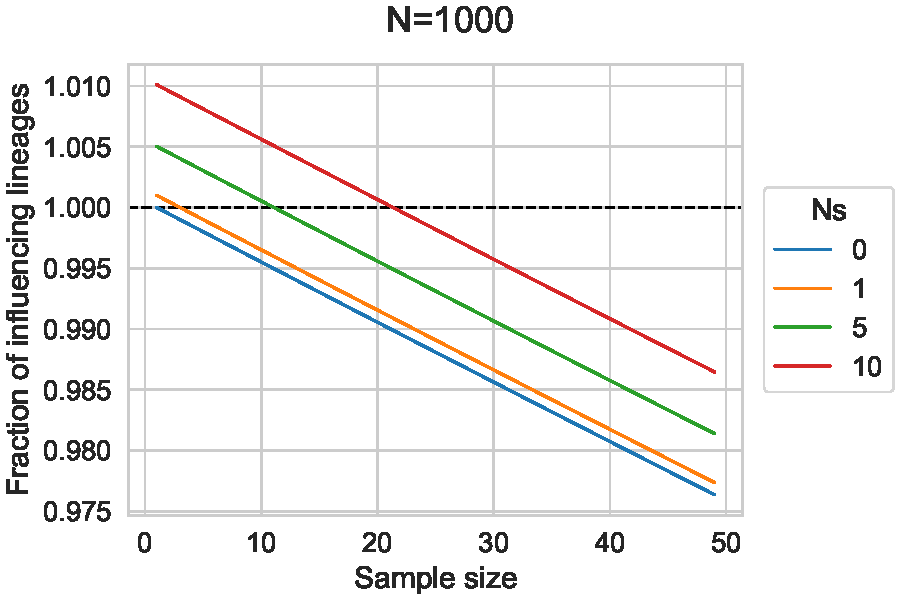
\includegraphics{fig/critical_sample_size.pdf}
  \caption{Critical sample size for different selection coefficients. The $Y$ axis shows the
    fraction of parental lineages over the sample size, $\frac{r}{n}$, each line corresponds to a
    different selection coefficient. Above $\frac{r}{n}\ge 1$, selection dominates, below -- drift.
    The critical sample size, where the expected number of parental contributing lineages is smaller
    than the sample size is well-approximated by $2Ns$.}
  \label{fig:critical-sample-size}
\end{figure}


Using the same equation, we can track the expected number of used parental lineages back in time,
which we denote as $n_{t-1}$:

\begin{align}
  \label{eq:contributors-back}
  n_{t-1}=\frac{n_txs}{1-xs} - \frac{n_t^2}{2N}
\end{align}

We solve this recurrence going back in time 10,000 generations, producing figure
\ref{fig:bell-plot}. The equilibrium point is well-approximated by $2Ns$, shown as a dashed line
here. This is the same as solving equation \ref{eq:critical-sample} explicitly. Non-withstanding of
the starting sample size, we converge to the equilibrium relatively quickly.

\begin{figure}
  \centering
  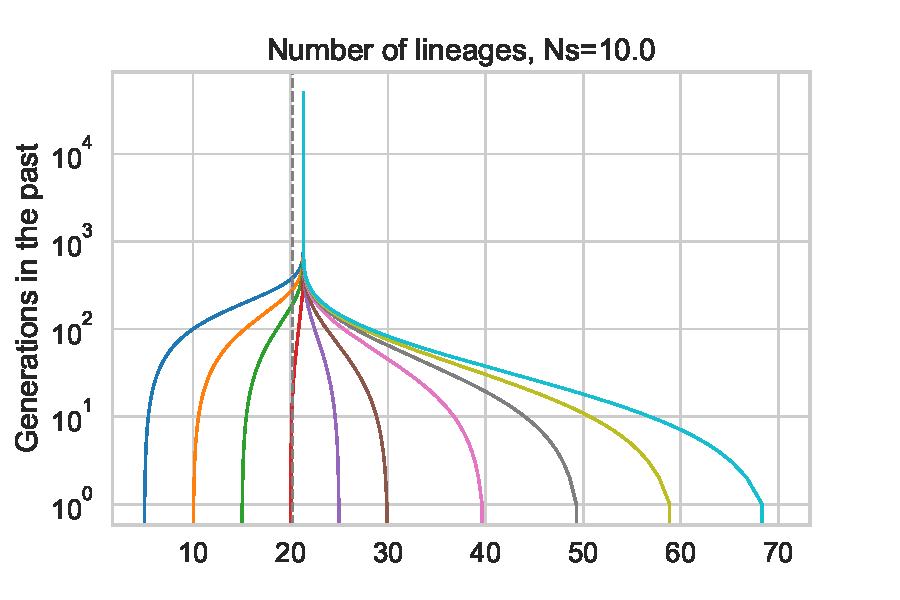
\includegraphics[]{fig/bell-plot.pdf}
  \caption{Expected number of contributing parental lineages back in time. Starting at a given
    sample size, the number of contributions is tracked with align \ref{eq:contributors-back}.
    The $Y$ axis shows time on a logarithmic scale, $X$ axis is the sample size. $N=1000$, $Ns=10$.}
  \label{fig:bell-plot}
\end{figure}


\subsection{Distribution of number of contributing lineages}
\label{subsec:distribution}

We now construct a probability distribution of the number of contributing lineages one generation
into the past.

The number of parental lineages used by drift can be modelled by the modified occupancy
(Arfwedson) distribution \citep{Wakeley2009,ONeill2019,JohnsonEtAl2005}. This is given by:

\begin{align}
  \label{eq:occupancy}
  P(\mathcal{R}=r|\mathcal{G}=g) = \frac{S_2(g,r) N!}{(N-r)! N^g}
\end{align}

where $S_2(g,r)$ is a Stirling number of the second kind, which is the number of ways to partition
$g$ objects into $r$ categories ($g$ gametes produced by $r$ parents). A typical statement of the
occupancy distribution is that we have $N$ urns and $g$ colored balls, and we want to know the
probability that exactly $r$ of the urns will be occupied (see \cite{JohnsonEtAl2005} section 10.4
for a thorough treatment). In our case, $N$ is the population size, urns correspond to the parents,
colored balls to gametes. Note that the under drift, the number of parents will be smaller or equal
to the number of gametes $r \le g$. The expectation of this distribution is given by equation
\eqref{eq:drift-expectation}.

The occupancy distribution is not simple to evaluate, but good performance can be achieved by
pre-computing a table of reduced occupancy numbers, using the algorithm of \cite{ONeill2019}.

As stated before, the number of lineages sampled under selection is described with a negative
binomial distribution. Unlike \ref{eq:neg-binom-fail}, however, we are now looking for the total
number of lineages sampled, not simply the number of failed trials. In this parameterization, the
probability of the negative binomial is given by:

\begin{align}
  \label{eq:neg-binomial-trials}
  P(\mathcal{G}=g|n) = \binom{g-1}{n-1}(1-xs)^n(xs)^{g-n}
\end{align}

Here, the number of gametes can be larger that the sample size $n \le g$, if selection is present
($s<0$).

Combining the two distributions together through \ref{eq:conditional}, we get:

\begin{align}
  \label{eq:lineages-in-past}
   Pr(\mathcal{R}=r|n) = \sum_{g=1}^{\infty} \frac{S_2(g,r) N!}{(N-r)! N^g} \binom{g-1}{n-1}(1-xs)^n(xs)^{g-n}
\end{align}

Unfortunately, this distribution does not have a simple analytical form. In certain parameter
regimes, this can be approximated by the normal distribution \citep{JohnsonEtAl2005,ONeill2019},
which we describe in the next section.

Figure \ref{fig:sampling-dist} shows the distribution of the number of contributing parental
lineages for several selection coefficients for a sample $n=20$. In the absence of selection, the
distribution has zero probability above $n=20$, as no extra lineages can be sampled. As the strength
of selection is increased, we begin requiring larger number of lineages. At the equilibrium point
($Ns=10$, \eqref{eq:critical-sample}), the distribution is symmetric.

\begin{figure}
  \centering
  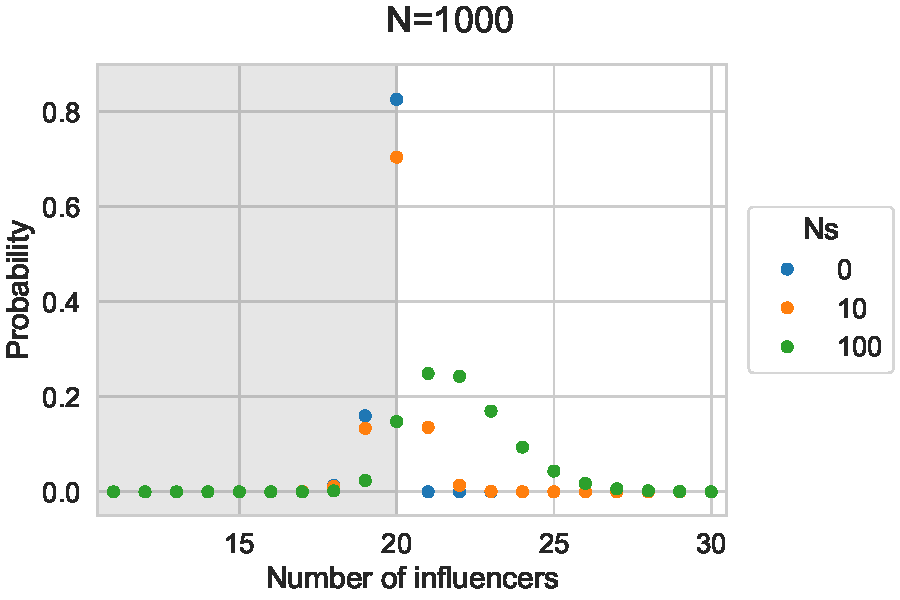
\includegraphics[]{fig/sampling-dist.pdf}
  \caption{The distribution of the number of parental contributing lineages one generation into the
    past ($n=20$, $N=1000$). Shaded area shows the drift-dominated regime, where the number of
    lineages is smaller than the sample size.}
  \label{fig:sampling-dist}
\end{figure}

We note that at the critical sample size, the probability that we will have a sufficient number of
lineages is only $50\%$. In order to guarantee that drift will out-pace selection, we can calculate
the cumulative distribution - Figure \ref{fig:cumulative-dist}. This shows that a sample size in
which the majority of lineages are accounted for can be substantially larger than the critical
sample size of equation \eqref{eq:critical-sample}. To derive a convenient expression, we turn to
the normal approximation in the next section.

\begin{figure}
  \centering
  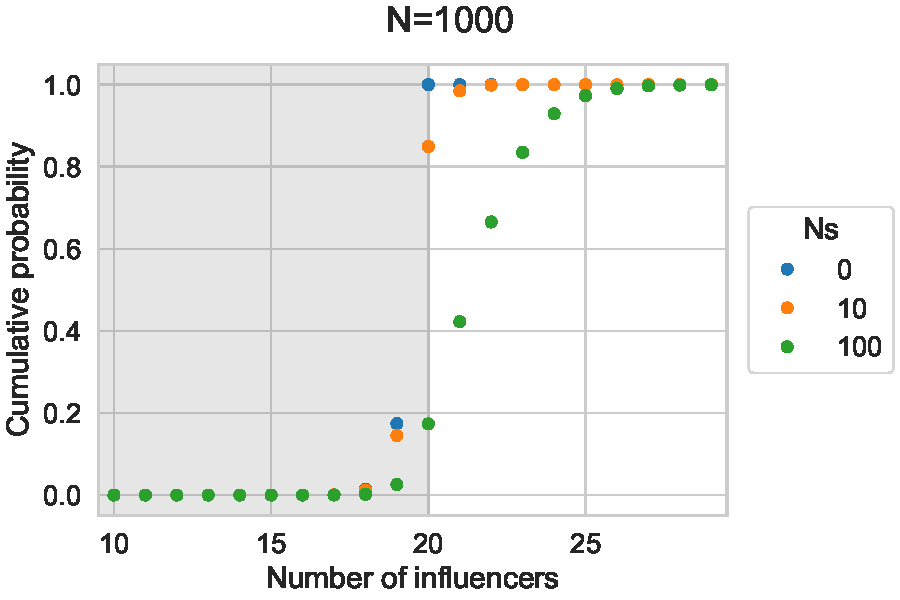
\includegraphics[]{fig/cumulative-dist.pdf}
   \caption{The cumulative distribution of the number of parental contributing lineages one generation into the
    past ($n=20$, $N=1000$). Shaded area shows the drift-dominated regime, where the number of
    lineages is smaller than the sample size. \ikcomment{This should be a two-panel with the
      previous figure}}
  \label{fig:cumulative-dist}
\end{figure}

\subsection{Normal approximation}

Finally, we can construct a normal approximation to the distribution of the number of contributing
lineages. The occupancy distribution is approximated by the normal \citep{ONeill2019} when $n \ll N$.
Likewise, the number of failures (eq. \eqref{eq:neg-binom-fail}) before a given number of successes,
can be approximated by the normal distribution. In the case of large population size, as required by
the approximation of the occupancy by the normal, we can approximate the total number of
contributing lineages as the sum of lineages contributed by the two distributions. The random
variable which is a sum of two normally-distributed random variables is also normal, with
$\mu=\mu_1+\mu_2$ and $\sigma^2 = \sigma^2_1 + \sigma^2_2$. By combining the required expectations
and variance, we find that the normal approximation then has the form:

\begin{align}
  \label{eq:normal-approximation}
  Pr(\mathcal{R}=r|n) \approx \mathcal{N}( \mu &= \left[(s n)/(1 - s) + N (1 - (1 - 1/N)^n)\right],\\
  \sigma &= \sqrt{N \left((N-1) \left(1-\frac{2}{N}\right)^n+\left(1-\frac{1}{N}\right)^n-N\left(1-\frac{1}{N}\right)^{2 n}\right)+\frac{n s}{(1-s)^2}})
\end{align}

Figure \ref{fig:normal-approximation} shows the quantiles of the normal approximation. We see that
up to $99\%$ of the lineages will be contained within the sample of 200 with $Ns=20$. Larger
percentiles will require larger sample sizes.

\begin{figure}
  \centering
  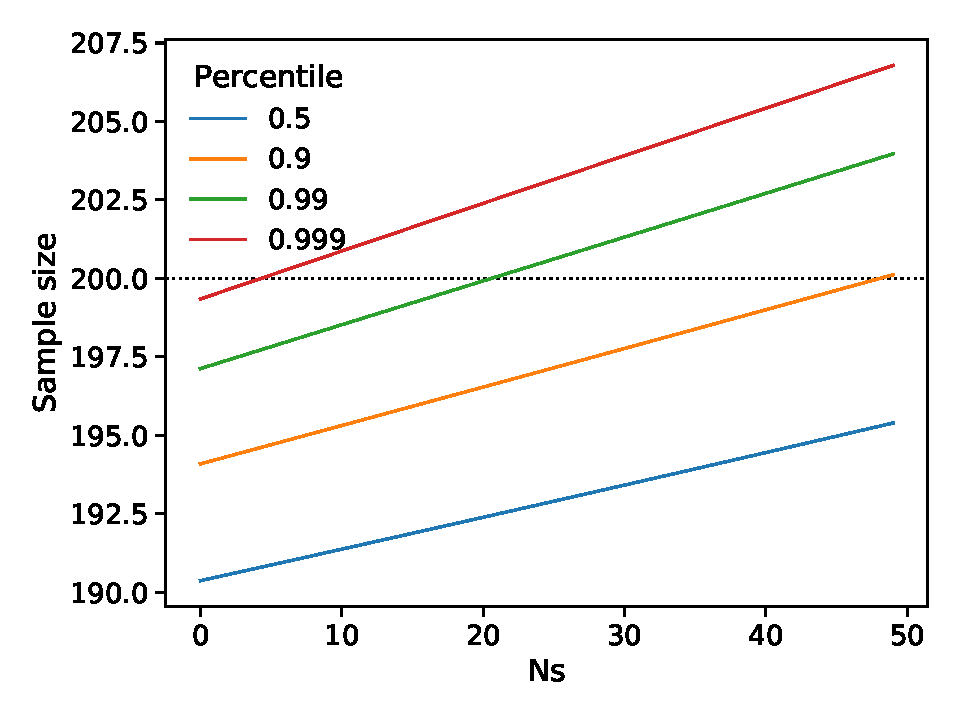
\includegraphics[]{fig/quantile.pdf}
   \caption{The quantile function of the closure of the sample. Each line corresponds to different
     percentile of the normal approximation. Black dashed line shows the reference sample size $n=200$.}
  \label{fig:normal-approximation}
\end{figure}


\section{Conclusion}
\label{sec:conclusion}

Classically, the coalescent considers models in the absence of natural selection. Since selection
can increase the number of contributing lineages back in time, the coalescent can no longer be
represented by trees, but instead acquires a graph structure. The ancestral selection graphs
\citep{KroneNeuhauser1997} deal with this in the limit of large population size ($N$).

The large population size approximation implies that the sample size $n$ is much smaller than the
whole population ($n \ll N$), so it is unlikely that more than one coalescent event will happen per
generation. However, recent work \citep{BhaskarEtAl2014,NelsonEtAl2019} pointed out that this
assumption is unreasonable with sample sizes pertinent to modern experiments. As a results, models
that consider multiple coalescent events per generation are gaining increased relevance in the
field \citep{FlemmingtonVoitCoalescentPapers}.

In this work we show that increasing the sample size has another unexpected consequence. As sample
size increases, the larger number of lineages needed due to selection can be masked by coalescent
events. In this sense, the large sample size rescues the model from effect of selection. This means
that recursion equations needed to calculate sample properties are asymptotically closed with large
population size.

At first approximation, $2Nsx$ is a critical sample size, where the decrease of lineages due to
coalescent back in time out-competes the increase due to selection (eq. \eqref{eq:critical-sample}).
Further, we derive the full probability distribution for the number lineages needed with given
selection coefficient and sample size (eq. \eqref{eq:lineages-in-past}). Unfortunately, the
distribution does not have a closed form, so we derive a normal approximation to the number of
lineages that contribute to a sample (eq. \eqref{eq:normal-approximation}). The normal approximation
then allows us to get a quantile function that we use to find if the model preserves closure with
some confidence level.

This work has several implications. First, we can combine the model described here with the
jackknife approximation \citep{JouganousEtAl2017}. This will allow us to construct a more robust
inference framework that can account for large sample size and strong selection.

Further, the results here suggest that effect of weak selection may be detectable in studies with
large sample sizes. This may open up a way for new investigations of natural selection in population
genetics.

\section{Appendix}

\ikcomment{TODO}


\bibliography{disco}

\end{document}
